\documentclass{article}
\usepackage{caption}
\usepackage{subcaption}
\usepackage{graphicx}
\usepackage{tikz}
\usepackage{tikzsymbols}
\usetikzlibrary{calc}
\usepackage{float}
\usepackage{pdflscape}
\usepackage{geometry}
\geometry{a4paper, landscape, margin=1cm}
\pagestyle{empty}

\def\centerarc[#1](#2)(#3:#4:#5){\draw[#1] ($(#2)+({#5*cos(#3)},{#5*sin(#3)})$) arc (#3:#4:#5);}

\begin{document}
	\centering
	\begin{figure}[H]
			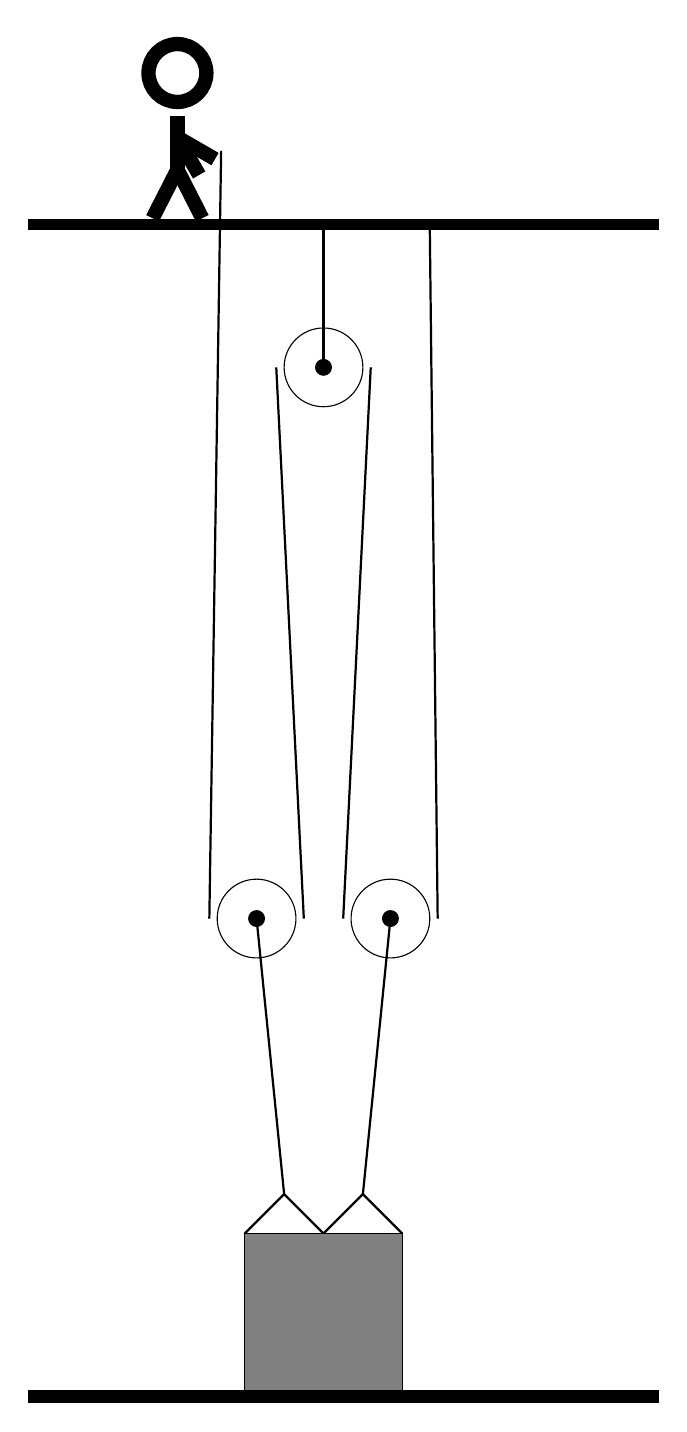
\begin{tikzpicture}
				%%%%% START %%%%%
								
				\draw[fill=black] (-2, 11.75) rectangle (6, 11.88);
				
				\draw (0.9, 3) circle (0.5);
				\draw[fill=black] (0.9, 3) circle (0.1);
				
				\draw (1.75, 10) circle (0.5);
				\draw[fill=black] (1.75, 10) circle (0.1);
				\draw[thick] (1.75, 10) -- (1.75, 11.75);
				
				\draw (2.6, 3) circle (0.5);
				\draw[fill=black] (2.6, 3) circle (0.1);
				
				\draw[thick] (2.6, 3) -- (2.25, -0.5);
				\draw[thick] (0.9, 3) -- (1.25, -0.5);
				\draw[thick]  (0.75, -1) -- (1.25, -0.5) -- (1.75, -1);
				\draw[thick]  (1.75, -1) -- (2.25, -0.5) -- (2.75, -1);
				\draw[fill=black!50] (0.75, -1) rectangle (2.75, -3);
				
				\draw[thick] (0.45, 12.75) -- (0.3, 3);
				\centerarc[thick](0.9, 3)(180:360:0.6);
				\draw[thick] (1.5, 3) -- (1.15, 10);
				\centerarc[thick](1.75, 10)(0:180:0.6);
				\draw[thick] (2.35, 10) -- (2.0, 3);
				\centerarc[thick](2.6, 3)(180:360:0.6);
				\draw[thick] (3.2, 3) -- (3.1, 11.75);
				
				\node at (-0.05, 13) {\Strichmaxerl[10][120][-30]};
				
				\draw[fill=black] (-2, -3) rectangle (6, -3.15);
				%%%%% END %%%%%
			\end{tikzpicture}
	\end{figure}	
\end{document}